\chapter{Optimization}\label{ch:optimization}

Consider a system which can take many different configurations.  Among the all configuration, we want find one configuration which best fits to a given criteria. For example, a molecule consisting of several atoms can take various geometric structures which are mechanically stable.  However, only one of them are the ground state and others are meta stable structures.  We want to find a structure that has the lowest energy.  That is an optimization problem.  In fact, the issue of protein folding has been a major optimization problem.\cite{protein_folding}  Another example, which we already encounter, is the least square fitting (See Chapter 11.)

To put the optimization problem in a mathematical form, the criteria is given as a function of configuration called fitness or cost function.  The best optimized configuration corresponds to the global minimum (or maximum) of the fitness function.  In this chapter we assume that the best fit corresponds to the global minimum of the fitness function.  Then, the optimization is an minimization problem.  We already learned several methods to minimize a function,  such as the steepest descent and conjugate gradient methods in Chapter 7.  However, when there are multiple minimums, those methods converges to a local minimum which is not necessarily the global minimum.  In the optimization problems, we want to find the global minimum. See Fig \ref{fig:local_minimum}.

\begin{figure}
\centering
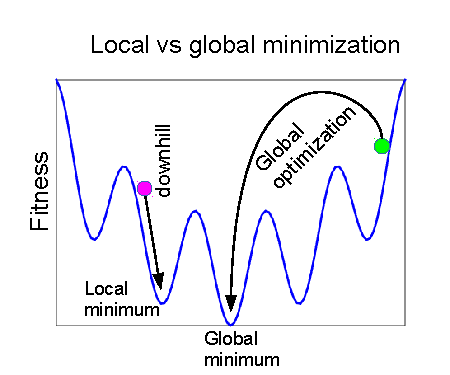
\includegraphics[width=2.5in]{19.Optimization/local_minimum.pdf}
\caption{Local minimization along the downhill goes down to the local minimum.  The global optimization must find the global minimum and thus the  search method must be able to go over the barriers between minimums.}
\label{fig:local_minimum}
\end{figure}

In Chapter 11, the least square fitting tries to fit a function to the given data by minimizing a $\chi^2$ function.  If the $\chi^2$ function is linear with respect to the parameters, there is only one minimum and thus the downhill method worked well.  On the other hand, if $\chi^2$ is a nonlinear function, then multiple local minima are possible.  Hence, the downhill method does not guarantee the best fit.

Finding a global minimum is not an easy task.  It turns out that the nature is doing it all time.  For example, when we heat up a  material and cool it down slowly, we obtain a crystal with fewer defects.  This procedure is called annealing.  However, if it is cooled down too quickly, the resulting crystal has a lot of defects.  It must be slowly cooled down to get a high quality crystal.  We can use a similar method in computer to find a global minimum.  The method is called \emph{simulated annealing}.  We ourselves are a result of global optimization though biological evolution, although we have not reach the global minimum yet (if it ever exists).   We can use the Darwin's evolution theory to find a global minimum. That method is known as \emph{genetic algorithm}.\cite{genetic_algorithm1,genetic_algorithm2}  In this chapter we learn these two methods.

\section{Fitness Functions}

In order to solve optimization problem numerically, we must write the problem in mathematical forms.  First, we need a configuration space which is a set of parameters $\{x_i\},\,(i=1, \cdots, N)$ to be adjusted and their domain $x_i \in [a_i, b_i]$.  We want to find a particular configuration $\{x_i^*\}$ that fits best to a given criteria. To express the crieteria in a mathematical form, we introduce a \textit{fitness} function. $F(\{x_i\})$.  It is also called \textit{cost} or \textit{loss} function.
The criteria is simply given by an inequality:
\begin{equation}
F(\{x_i^*\}) \le F(\{x_i\}
\end{equation}
which means $F(\{x_i^*\})$ is the global minimum.  Hence,  optimization is equivalent to finding the configuration corresponding to the global minimum of a fitness function.
An example of the fitness function is the $\xi^2$ function [see  Eq (11.18)].  

The fitness function is not unique and you can construct many different fitness functions for the same optimization problem.  All of them have the same configuration $\{x_i^*\}$ at the global minimum. We can utilize this freedom to construct a fitness function that is numerically easier to evaluate.  In fact, the evaluation of the fitness function consumes most of computation time during the minimization.Therfore, constructing a good fitness function saves significant amount of computing time.

On he other hand, we can also construct ill-conditioned fitness functions if we are not careful.  For example, when we want to find the lowest energy geometric structure of a molecule, a convenient fitness function is the potential energy of the molecule and the configuration is the coordinates of all atoms. We have to make it sure that the configuration is uniquely determined by the optimization procedure.  The potential energy is a function of the position of atoms.  If we treat all coordinates as the degrees of freedom, we cannot uniquely determine the position of the all atoms by minimizingthe  potential energy.  If we shift or rotate the molecule without changing its shape, the potential energy does not change.  Depending on the algorithm, the optimization procedure never stops and the molecule keeps rotating or sliding without changing the structure!
Removing the degrees of freedom with respect to the global translational and  rotation, the number of degrees of freedom to be determined for the $N$-atom system becomes $3N-6$ for $N\ge 3$. 

As a toy example, consider a pair of particles connected by a spring of natural length $\ell$ and spring constant $k$.  The potential energy of the system is given by
\begin{equation}
U(\mathbf{r}_1, \mathbf{r}_2) = \frac{k}{2} \left ( \left | \mathbf{r}_2-\mathbf{r}_1 \right | - \ell \right )^2.
\end{equation}
where $\mathbf{r}_i$ is a position vector of $i$-th particle.
Now, we want to find the lowest energy structure.  Then, $U(\mathbf{r}_1, \mathbf{r}_2)$ is the fitness function in the six dimensional configuration space.
The solution can be found immediately by direct inspection.  When the distance between two particles equals the natural length of the spring, the energy is exactly zero.  Since the harmonic potential energy cannot be negative, it is the optimum structure.  However, the solution is not unique since any rotation of the system gives the same potential energy.  Therefore, the minimum energy configuration is not a point in the six dimensional space.

To avoid the above issue, we place the particles on the $x$ axis. We limit the degrees of freedom to $x_1$ and $x_2$.  Other components of the position vectors are set to zero.  This prohibits the rotation of the system. The potential energy is 
\begin{equation}
U(x_1, x_2) = \frac{k}{2} \left (\left |x_1-x_2 \right |-\ell \right )^2.
\end{equation}
Now the configuration space is only two-dimensional.  The potential energy is plotted in Fig.  The dark blue corresponds to the configuration of low potential energy.  Notice that the minimum is a diagonal line and thus the minimum is not a unique point. This is because the translation displacement of the system does not change the potential energy.  This problem can be avoided, if we fix the position of one particle and optimize the position of the other particle only. Letting $x_2=0$, the potential energy is just
\begin{equation}
U(x_1) = \frac{k}{2} \left ( \left | x_1 \right | - \ell \right )^2
\end{equation}
with only one degree of freedom.  Furthermore, we assume $x_1>0$ since the potential does not depend on the sign of $x_1$. The optimized configurations are clearly $x_1=\ell$, which we expected at the first place.  It is possible to ask computers to do all these reduction of degrees of freedom.  However, the coding becomes complicated in many cases. It is better to use our own brain to remove the difficulty when possible. 

\bigskip
\begin{example}\label{ex:global_harmonic_coupling}
Consider N particles connected to eac other by identical springs.  The spring has a natural length $\ell$ and a spring constant $k$.   Using the position vectors $\mathbf{r}_i, \quad i=1,\cdots,N$, the potential energy is usually written as
\begin{equation}\label{eq:U_all_pairs}
U(\mathbf{r}_1, \mathbf{r}_2, \cdots, \mathbf{r}_N) = \sum_{j>i} \frac{k}{2} (\left |\mathbf{r}_j-\mathbf{r}_i \right | - \ell )^2.
\end{equation}
Here $\sum_{j>i}$ means the summation over all possible pairs of particles without double counting.  In this expression, the parameters are three components $x_i$, $y_i$, and $z_i$ of $\mathbf{r}_i$ for each particle and thus there are $3N$ parameters to be adjusted. 

We already discussed the dimer ($N=2$).  For $N=3$ and $4$, it is easy to see that an equilateral triangle and a tetrahedron are the minimum energy structures, respectively since every pair has the same distance. However, the minimum energy structure for $N \ge 5$ is not obvious.  Is a cube the global minimum for $N=8$?

Searching for the global minimum with respect to all coordinates $\mathbf{r}_i$ is not
a good idea.  We need to remove the rotational and translation degrees of freedom.  We can always put the atom 1 at the origin of coordinate ($\mathbf{r}_1=0$) to stop the translational motion.  Now, how do we stop the rotation?   If we place any three atoms on a fixed plane. For simplicity we place the fist three atoms on the $xy$ plane by 
\begin{equation}
\mathbf{r}_1=(0,0,0), \qquad \mathbf{r}_2=(x_2,0,0), \qquad \mathbf{r}_3 = (x_3, y_3, 0)
\end{equation}
Since six degrees of freedom are now fixed to zero, we need to optimize $3N-6$ degrees of freedom.

We have used Cartesian coordinates of the atoms to describe the geometric structure.  There are other methods.  Among them, the Z-matrix is popular. It uses the distance between atoms and dihedral angles specifying the relation of three atoms.  It has no translational nor rotational freedom. The Z-matrix is convenient when we optimize molecular geometries.\cite{z-matrix}   The Z-matrix can be converted to the Cartesian coordinates. 

  
\end{example}

\section{Simulated Annealing}

\begin{figure}
\centering
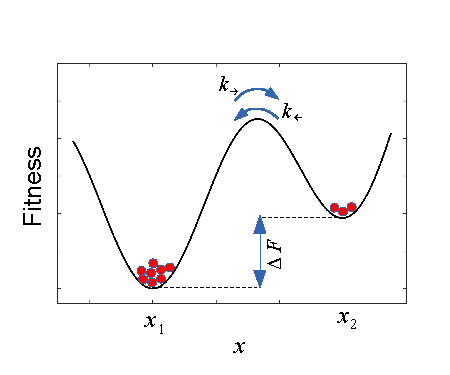
\includegraphics[width=2.5in]{19.Optimization/sa.pdf}
\caption{The particles can jump between two minimums over the barrier. The transition rate $k_\rightarrow.$ from the deeper minimum at $x_1$ to the shallow minimum at $x_2$ is smaller than the other direction of transition rate $k_\leftarrow$.  Its ratio is given by $k_\rightarrow/k_\leftarrow = \me^{-\Delta F/T}$. The particle current is $N_1 k_\rightarrow - N_2 k_\leftarrow$ where $N_i$ is the number of particle in the basin of $i$-th minimum. At thermal equilibrium particle current must vanish (detailed balance). Therefore, $N_1/N_2 = k_\leftarrow/k_\rightarrow > 1$.  At thermal equilibrium, more particles are found in the deeper minimum than the other.}
\label{fig:sa}
\end{figure}

In metallurgy,  defects in a material are removed by raising temperature to a certain level and cooling it down gradually.  The procedure is known as annealing.  At high temperature the atoms diffuse rapidly.  When the temperature is reduced, the atoms settle down to a stable state. When cooled slowly enough, the most stable state is formed.  Ideally it is a defect-free crystal.  Mathematically speaking, the annealing process can be understood as global minimization of the system energy since the formation of defects costs some energy. 

Perhaps, we can utilize the annealing mechanism to solve other optimization problems, even purely mathematical optimization problems unrelated to physics.  In order to imitate the  thermodynamics process of annealing, we construct a fictitious thermodynamic system.  Consider the fitness function $F(\mathbf{p})$ as ``energy'' of the system and the configuration $\mathbf{p}=(x_1, \cdots, x_N)$ as ``coordinates'' of the atom. 
Note that we have only one atom and the coordinate space is $N$-dimensional. We further introduce fictitious ``temperature'' $T$.  At ``thermal equilibrium'', the probability to have a configuration $\mathbf{p}$ is assumed to be proportional to $\me^{-F(\mathbf{p})/T}$, analogous to the Boltzmann distribution.  If we ``anneal'' this fictitious thermodynamical system, we should be able to find the global minimum of the fitness function.  In the following discussion, we use words like energy or temperature for convenience but they are not real energy or temperature.  

Now, we let the atom  diffuses at a fixed temperature.
In Chapter 15, we learned the Monte Carlo simulation of thermal equilibrium states using Metropolis algorithm.  The microscopic state changes randomly according to the Boltzmann distribution.  We can use the exactly same algorithm to sample the configuration space.
Note that the atoms not always go down hill in the energy.  The Metropolis method allows the atoms to climb  up the hill as long as it satisfies the detailed balance.  Hence, the atoms are not confined in a basin of a local minimum.    Let $P_i$ the probability of finding atoms at the $i$-th minimum.  The detailed balance suggests that when the system is at thermal equilibrium,
\begin{equation}\label{eq:sa_detailed_balance}
\frac{P_i}{P_j} = \me^{-(F_i-F_j)/T}
\end{equation}
where $F_i$ is the value of the fitness function at the $i$-th minimum.  Equation (\ref{eq:sa_detailed_balance}) indicates that if $F_i> F_j$, then $P_i<P_j$.  This means that the atoms are in the deeper energy minimum more often than the shallow one. Figure \ref{fig:sa} illustrates the case where there are two minimums.  
If temperature $T$ is lowered, the difference between $P_i$ and $P_j$ increases and it easier to identify the global minimum configuration. On the other hand, if temperature is too low, it takes a long time to reach thermal equilibrium.  Therefore, we start with a considerably high temperature and keep the temperature constant until the thermal equilibrium is established.  Then, we slowly lower temperature so that system remains in thermal equilibrium until the global minimum is clearly identified.
This optimization procedure is called \textit{simulated annealing}.  

It is important to note that we identify the global minimum based on the probability distribution $P_i$.  To find the probability distribution, we must have a population of atoms $(\mathbf{p}_1, \cdots, \mathbf{p}_K)$ each of which is independently annealed.  If the population size $K$ is too small, the statistics is not accurate and we may not have enough resolution to find the global minimum.  

Theoretical speaking, the simulated annealing can find the global minimum configuration accurately by lowering temperature to absolute zero.  However, it is not practical.  When the basin of the global minimum is identified, the steepest descent or other minimization method based on the gradient is much more efficient to go to the exact minimum. See Section 7.4
\bigskip
\begin{myalgobox}
\Algorithm{Simulated Annealing}\label{algo:sa}

\medskip
\begin{minipage}{5.5in}
\small
\begin{enumerate}
\item Define a fitness function $F(\mathbf{p})$ where $\mathbf{p}=(x_1, \cdots, x_N)$ is a vector of size $N$ in the given configuration space.
\item Set an initial population $(\mathbf{p}_1, \cdots, \mathbf{p}_K)$ at random .
\item Set an initial temperature $T$.
\item Repeat the following Metropolis method $N_\text{th}$ times for all $i$.
\begin{enumerate}
\item Pick a new configuration $\mathbf{p}^\prime_i = \mathbf{p}_i + \delta \mathbf{p}_i$ where $\delta \mathbf{p}_i$ is a small random vector.
\item Evaluate the change in the fitness function $\Delta F_i = F(\mathbf{p}^\prime_i) - F(\mathbf{p}_i)$.
\item Generate a uniform random number $r$ between 0 and 1.
\item If $\me^{-\Delta F_i} > r$, accept the new configuration and let $\mathbf{p}_i=\mathbf{p}^\prime_i$. 
\item  Otherwise reject the new configuration and go to 4(a) until a new coordinate is found.
\end{enumerate}
\item Reduce the temperature  according to a cooling schedule.  If $T<T_\text{c}$, it is done where $T_\text{c}$ is a cut of temperature.  Otherwise go to Step 4 with the new temperature.
\item Find the basin of the minimum that has most populated.  That minimum is the global minimum.
\end{enumerate}
\end{minipage}
\end{myalgobox}

\bigskip
\begin{example}[One-dimensional global minimum by simulated annealing]\label{ex:sa}

\medskip
\noindent
We want to find a global minimum of a function 
\begin{equation}
f(x) = 3-3\cos(2x)+0.2 x^2
\end{equation}
This function is the fitness function which depends only on one variable.  We can interpret it as an atom in one-dimensional potential well. We use a population of eight atoms to get a statistics.  Eight is not big enough in general but it works OK for this problem.
Program \ref{prog:sa} implements Algorithm \ref{algo:sa} and solve this problem.  The result is shown in Fig. \ref{fig:sa_example1}.  As shown in Fig. \ref{fig:sa_evolution}, temperature is lowered exponentially over 200 steps.  At each step, the system was thermalized over 2000 Metropolis steps.  The lowest value of the fitness (red line) indicates that the atoms are jumping in and out from the minimums until temperature approaches 0.5.  Figure \ref{fig:sa_fitness} suggests that five out of eight atoms are found in the global minimum.  Two other local minimums are occupied.  No atom is found at the remaining minimums.  Therefore, the global minimum has the highest probability.


\begin{figure}
	\centering
	\begin{subfigure}{0.45\textwidth}
		\centering
		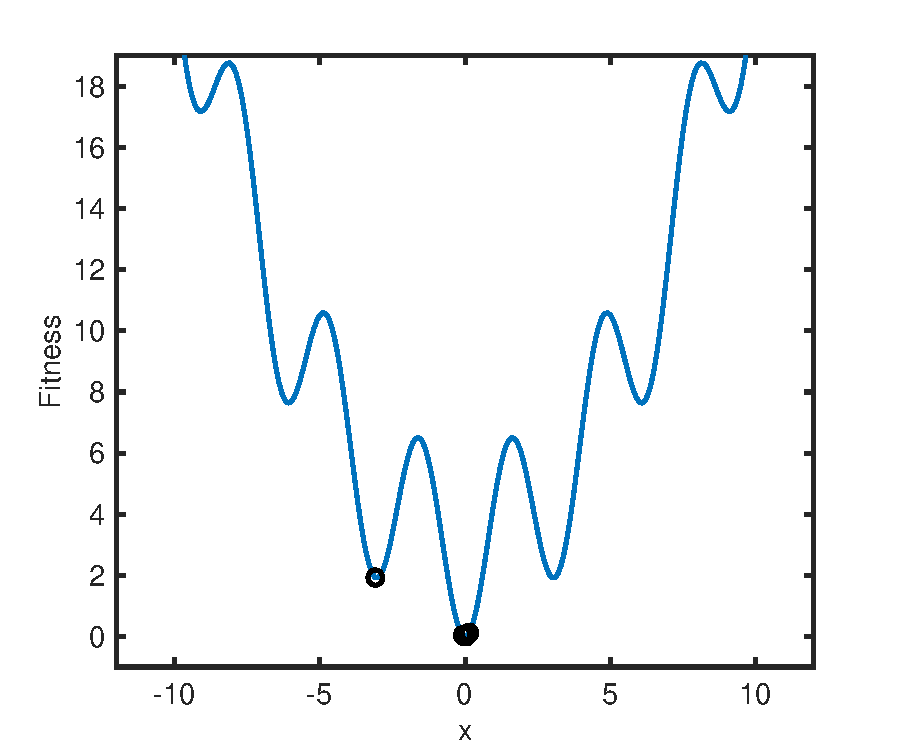
\includegraphics[width=2.4in]{19.Optimization/sa_fitness.pdf}
		\caption{The final population.}
		\label{fig:sa_fitness}
	\end{subfigure}
	\begin{subfigure}{0.45\textwidth}
		\centering
		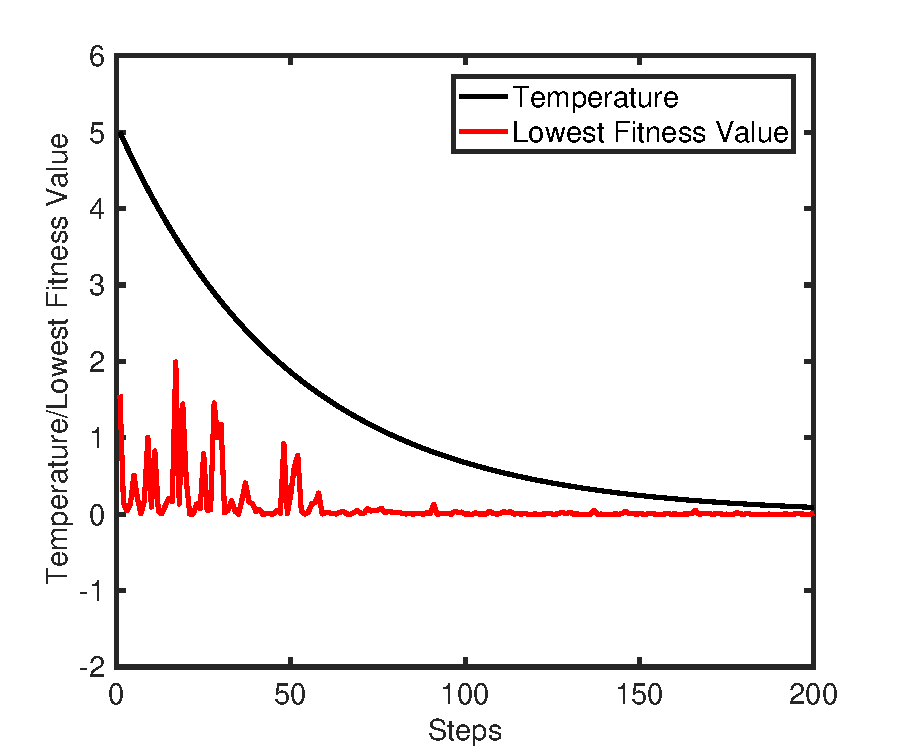
\includegraphics[width=2.4in]{19.Optimization/sa_evolution.pdf}
		\caption{Evolution of temperature and the lowest value of the fitness.}
		\label{fig:sa_evolution}
	\end{subfigure}
\caption{Searching a global minimum by the simulated annealing method.  Eight samplers explore the landscape of the fitness function based on Metropolis method. (a) The fitness landscape shows several local minimums and the rather high barrier between minimums. At the end of the annealing three out of eight samplers are trapped in the basin of the global minimum.  The remaining samplers are trapped in local minimums. (b)  The evolution of the temperature indicates the exponential cooling schedule. The lowest fitness values among the population randomly changes when the temperature is high. As temperature is reduced, the samples are trapped in basins of minimums and the lowest fitness value no longer changes significantly.}
\label{fig:sa_example1}
\end{figure}

\end{example}

\noindent
\section{Genetic Algorithm}

\begin{figure}
\centering
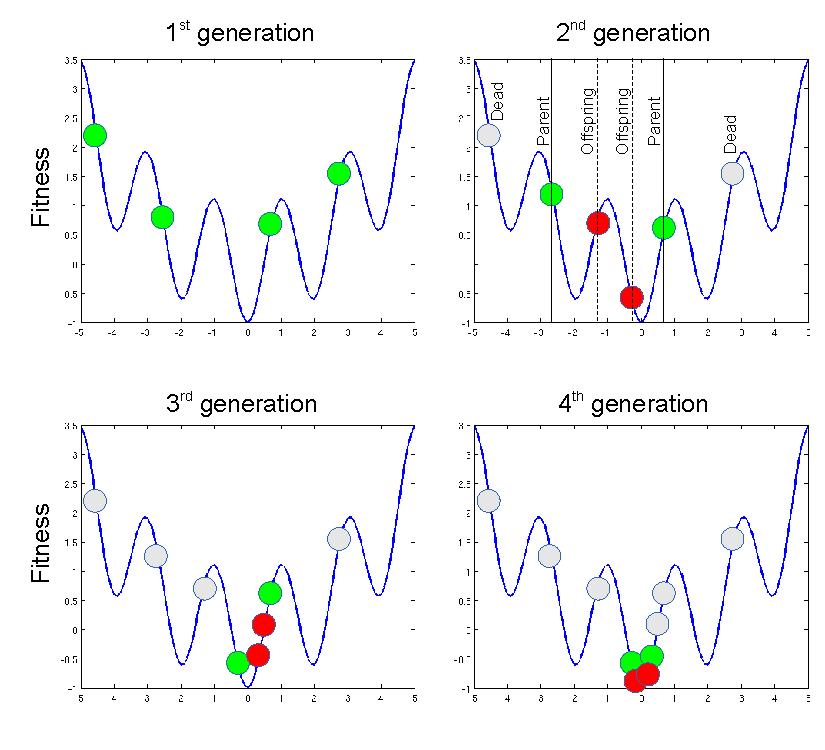
\includegraphics[width=3.5in]{19.Optimization/ga-diagram1.pdf}
\caption{Schematic diagram of genetic algorithm. Evolution of a species which has only one gene. The population consists of four individuals. The horizontal axis indicates \textit{genotype}. The genes of the first generation are chosen at random.  A half of the population die due to the high fitness values. The remaining two individuals become a bleeding pair and generate two children whose genotype is between parent's gene.  Now the size of population is back to four. The same process is repeated.  The third and forth generations are shown. The unfit individuals die and the survived individuals are localized near the global minimum.}
\label{fig:ga_diagram1}
\end{figure}
\begin{figure}
\centering
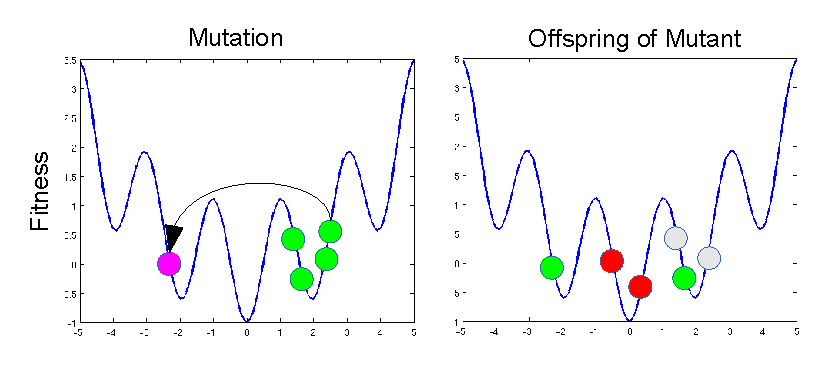
\includegraphics[width=3.5in]{19.Optimization/ga-diagram2.pdf}
\caption{Effects of mutation:  The left panel shows that all four individuals are trapped in the basin of a local minimum. Their children will be also in the same basin. To avoid this situation, an individual jumps to a random location (pink). This is the mutation.  After the mutation, the individuals with higher fitness values die.  If the mutated individual happened to fit better than others, it survives.  The children born from the mutant are now outside of the basin of the local minimum.  Now the four individuals are spread over three different minimums and thus the diversity of the population increased by the mutation.}
\label{fig:ga_diagram2}
\end{figure}

Evolution of biological systems roughly speaking follows the Darwin's evolution theory. Consider a population consisting of many diverse individuals. Some of them do not fit to the living conditions and die.  The survivors make offspring which inherits their parent's genes and fits well to the same living conditions.  After many generations, most members in the population well fit to the conditions and survive until the condition changes.  If all members of the population are very similar, they would not survive when the living condition changes.  However, the species survives because mutation keeps the diversity in the population.  Upon the change of the conditions, only a few members may survive and their offspring tends to survive.  After several generations, the size of the population recovers.

Learning from this remarkable process, we utilize the selection and mutation rules to navigate the population toward the minimum of the fitness function.  After certain generation, their descendants populated at the global minimum (the best place to live).  
We consider again the configuration $p=\{x_i\}$ as before.  By analogy from the biological evolution, $p$ represents an individual in the population and the parameters $\{x_i\}$ are its genes.  A population consists of $N$ individuals ($p_1, \cdots, p_N$).  A fitness function $F(p)$ determines if the individual fits to the current living condition.  The individual fits better when the value of the fitness is smaller.  The optimal genes $\{x_i^*\}$ corresponds to the global minimum of the fitness.

Now we construct the fictitious evolution process.  There are many possible evolution processes.  He we consider a simple one.
First, we set a selection rule.  The individuals with higher fitness values are considered unfit and a half of population whose fitness value is above the median die.  Figure \ref{fig:ga_diagram1} illustrates the evolution process.  Four individuals are generated at random.  This is the 1st generation.  Two individuals with high fitness values die (colored grey in the second generation diagram).
At this point only two individual survives in the population.



After death of unfit individual, the population needs to make offspring.  To do so, first we need to pair two individuals.  This is based on the popular form of life on the earth.  In a fictitious biological world, it is in principle possible that more than two individuals get married and make offspring inheriting genes from all parents.  For simplicity, we assume that a couple of individuals are mated. As a simplest mating rule,  we just make a pair at random. Algorithm of random paring will be discussed shortly after the overview of the genetic algorithm is presented.

Once a couple is formed, they make two babies so that the population is back to the original size.  We need a rule to determine the genes of the babies. There are many other possible rules depending on the type of optimization problems.
Here we use a simple formula:
\begin{equation}
p_\text{baby1} = \xi p_\text{adult1} + (1-\xi ) p_\text{adult2}, \qquad p_\text{baby2} = (1-\xi) p_\text{adult1} + \xi p_\text{adult2}
\end{equation}
where $\xi$ is a uniform random number between 0 and 1.  This rule make it sure that the genes of the babies are between the genes of the two parents.  The fitness of the new genes is not necessarily lower than that of the parents.

After the population recovers its original size, some of the individuals undergo mutation. Again, there are many different way to introduce mutation.  A simple example uses a mutation rate $k_\text{mutation} \in (0,1)$.  Generate a uniform random number $r$ for each individual.  If $r<k_\text{mutation}$ then mutation takes place and change the genes of the individual also at random. 
Figure \ref{fig:ga_diagram2} shows how mutation helps. When all individuals in the population are trapped in a local minimum.  The offspring they generates also in the same minimum.  However, if mutation happens, the offspring escape from the minimum. Mutation is important to keep the diversity in the population. Otherwise, the whole population could trapped in a local minimum. 
Usually we use a different mutation rate for each generation. In some cases, a proper variation of the mutation rate increase the computation time dramatically.

Now we completed the formation of a new generation.  By repeating the procedure, gradually the population drift to the global minimum. See the third and forth generations in Fig. Figure \ref{fig:ga_diagram1}.  All unfit individuals are dead and those who have lower fitness survives in the global minimum.



An important and difficult question is when we stop the procedure.  We monitor the lowest fitness value among the population.  If that does not change for many generations, we hope that one of the individuals arrived at the global minimum.  The waiting time must be sufficiently long so that mutation happens at least several times to make it sure that the population is not stuck in a local minimum.
Algorithm \ref{algo:ga} summarizes the procedure. Like the simulated annealing method, the genetic algorithm identify the basin of the global minimum within a reasonable computing time but takes too long to reach the true global minimum. AS soon as we find the basin of gloabl minimum we can use steepest descent or other minimization methods based on the gradient of the fitness function. 


Now, we introduce an algorithm of random paring.  Consider individuals with an ID number 1 through $M$.  We want to make $N/2$ pairs at random.  If $N$ is not an even integer, there is one individual who will not have a mate and thus it cannot produce offspring.  The random pairing is equivalent to a problem of random permutation. For $N=4$, we have a sequence $\{1 2 3 4\}$.  When it is randomly permuted, we obtained, for example,  $\{4 1 3 2\}$.  Then, we make pairs in the order of the permuted sequence.  For this example, (4,1) and (3,2) are the two couples.   There is a simple algorithm to generate random permutation of 
integers from 1 through $N$.  Figure \ref{fig:knuth_shuffle} shows an algorithm called the Knuth shuffle.  The rule is simple.  We are going to place integers from $1$ through $N$ in $N$ empty seats.   When we place $j$, we chose a seat at random between seat $1$ and  seat $j$.
If the seat is already occupied, the content of the seat will be relocated to seat $j$.  Just repeat this procedure from $j=1$ to $j=N$.
For $N=3$ (See Fig \ref{fig:knuth_shuffle}), we start with $j=1$.  There is only one allowed seat and thus $1$ go to seat 1. $j=2$ has two possibilities, seat 1 or 2.  Use a random number to choose one.  If seat is 2, just put 2 there since the seat is unoccupied.  If seat 1 is selected, put 2 there. and the previous occupant bumps out to seat 2.  For $j=3$, there are three seats.  Choose one at random.  If the selected seat is already occupied, put 3 there and the previous occupant bumps out to seat 3.  At the end, we have six different outcomes with equal probability.  Since the total number of permutation is $3!=6$, all of them are counted. The following code generates the random permutation. (MATLAB has a built-in function for random permutation, see help for \texttt{randperm(n)}.)

\begin{figure}
\centering
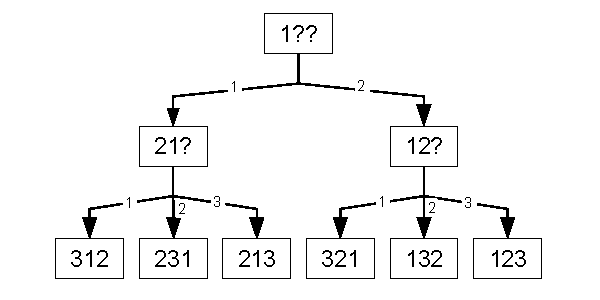
\includegraphics[width=2.5in]{19.Optimization/knuth_shuffle.pdf}
\caption{Knuth shuffle algorithm}
\label{fig:knuth_shuffle}
\end{figure}

\begin{center}
\begin{mybox}
\begin{verbatim}
for i=1:n
    j=ceil(rand(1)*i);
    p(i)=p(j);
    p(j)=i;
end
\end{verbatim}
\end{mybox}
\end{center}

\bigskip
\begin{myalgobox}
\Algorithm{Genetic Algorithm for continuous parameters}\label{algo:ga}

\medskip
\begin{minipage}{5.5in}
\small
\begin{enumerate}
\item Define a set of parameters  $p=\{x_1, x_2, \cdots, x_N\}$ which corresponds to the property of the individual $p$.
\item Define a fitness function $F(p) \equiv F(x_1, x_2, \cdots, x_N)$.  The fitness of the individual is evaluate by the fitness function.
\item Define a selection rule based on the fitness.  For example anyone whose fitness is larger than a cut off $F_c$ or the worst 20\% will be killed.
\item Generate an initial population consisting of $M$ individuals $\{p_1, p_2, \cdots, p_M\}$ at random.
\item Evaluate the fitness of each individual $F(p_i)$ and then determine which ones die based on the selection rule.
\item Pair survived individuals for mating at random.
\item Generates two offspring from each mating couples until the size population becomes $M$ again. (Deads are replaced with children.) The parameter values of the offspring will be
\[
p_\text{child 1} = p_i + \xi (p_j-p_i), \quad p_\text{child 2} = p_j + \xi (p_i-p_j)
\]
where $p_i$ and $p_j$ are their parents and $\xi$ is a uniform random number between 0 and 1.
\item Mutate some individual. Generate a uniform random number $\xi$. If $\xi < k_\text{mutation}$, then mutation occurs. Select an individual at random and change its parameter values at random.
\item Now we have a new generation of population.  Decide if some of them are at the global minimum of the fitness. If the lowest fitness does not change for many generations, we hope that at least some are at the lowest point.
\item If yes, stop the procedure. Otherwise, go to Step 4.
\end{enumerate}
\end{minipage}
\normalsize
\end{myalgobox}


\bigskip
\begin{example}[One-dimensional Global Optimization]\label{ex:ga}

We solve the same problem as Example \ref{ex:sa} but with the genetic algorithm this time.
First, we generate an initial population consisting of $N=32$ individuals $\{x_1, \cdots, x_{32}\}$, which is distributed uniformly random over the range of the variable $x$.   It is convenient if the number of individual is a power of 2.

Now we enter the selection phase. We evaluate the fitness of the individuals, $F_i=F(x_i)$ and then sort the individuals based on the fitness values
\begin{equation}
F_{x_{i_1}} \le F_{x_{i_2}} \le \cdots \le F_{x_{i_N}}
\end{equation}
We assume that upper 50\% of population die due to misfitting.  The individuals from $x_{i_{N/2+1}}$ to $x_{i_N}$ are dead.
There are many sorting algorithm.  Here we just use the sorting function built in MATLAB.  Many systems such as Linux provides various sorting functions.

Mating is the next step. Survivors from $x_{i_1}$ to $x_{i_{N/2}}$ pick their mate at random using the Knuth algorithm. 
Each mating couple produces two offspring so that the size population recovers from the death of misfit individuals.  The gen of the childrens are determined by the rule explained in Algorithm \ref{algo:ga}.

Final step is mutation.
Now, we have a new generation of the population with a certain diversity.  In this world, there is no age. The individual can survive forever as long as it fits to the living condition.  We repeat this procedure and after certain generations and the population will hopefully find a ultimate gene with which the fitness function takes the lowest value.  But when does it happen?  This is an big problem of the generic algorithm.  There is no general rule that guarantees the global minimum. If the whole population is stuck in a local minimum, they must wait until mutation brings some individuals out of the local minimum.  It might take a long time to escape from the local minimum.  A common method is to limit the waiting time $\tau$.  We check the lowest fitness $F_{i_1}$ for every generation.  If it does not change over the given waiting period.  We assume that $F_{i_1}$ is the global minimum.  The waiting period must be long enough that the mutation happens many time during the waiting period.  That is $\tau k\gg 1$.

Program \ref{prog:ga} implements the above algorithm and find the global minimum of the given function within the given range.  Simple selection, mating, inheritance, and mutation rules given in Algorithm \ref{algo:ga} is used. In particular, a fixed mutation rate is used.
Figure \ref{fig:ga} shows that the best gene within the population gets better as the generation goes on. After 20th generation, the improvement is no longer seen, suggesting that the global minimum is discovered.

\begin{figure}
\centering
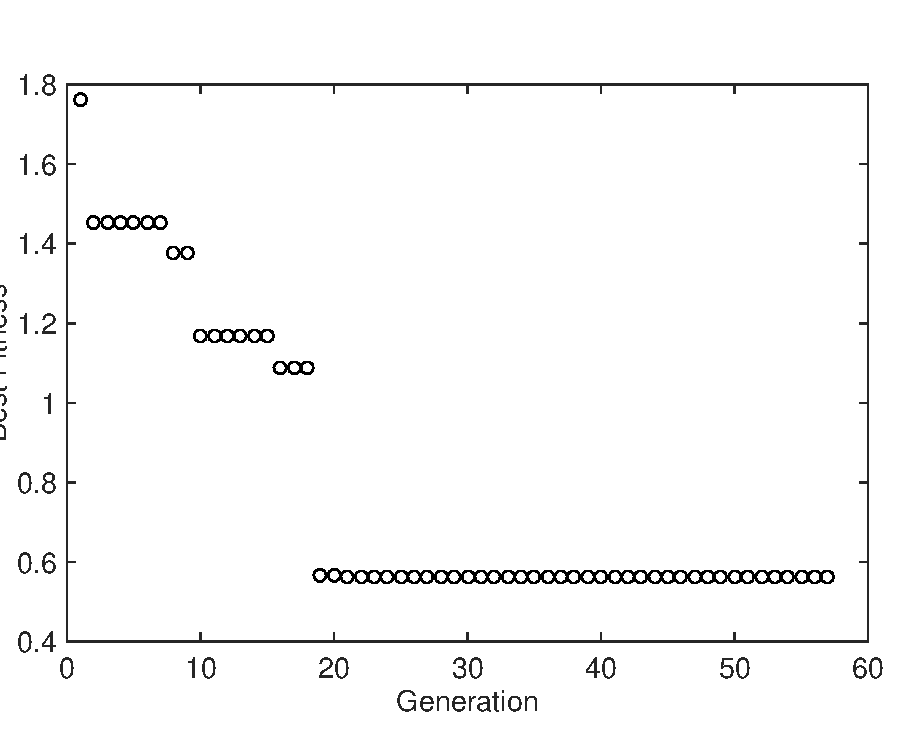
\includegraphics[width=2.5in]{19.Optimization/ga_evolution.pdf}
\caption{The evolution of the best fitness value.  The best gene of the population gradually improves as the generation moves on.  After 20th generation, the best fitness stays almost constant, indicating that the global minimum is discovered.} 
\label{fig:ga}
\end{figure}

\end{example}

\noindent
\section{Applications in Physics}

\noindent
\subsection{Fitting to Gaussian Distribution}\label{ex:ga_gauss}

\begin{table}
\centering
\caption{Data set for Gaussian distribution}\label{tbl:Gaussian}
\begin{tabular}{c|ccccccccccccc}
\hline
$x$&-1.98&-1.48&-1.00&-0.50&-0.02&0.51&1.019&1.52&1.99&2.52&3.00&3.52&3.99\\
$\bar{f}$&0.10&0.11&0.31&0.65&1.28&1.785&2.13&1.92&1.73&0.70&0.31&0.14&0.14\\
$\sigma$&0.14&0.11&0.15&0.18&0.18&0.12&0.11&0.10&0.16&0.15&0.10&0.17&0.18\\
\hline
\end{tabular}
\end{table}

\begin{figure}
\centering
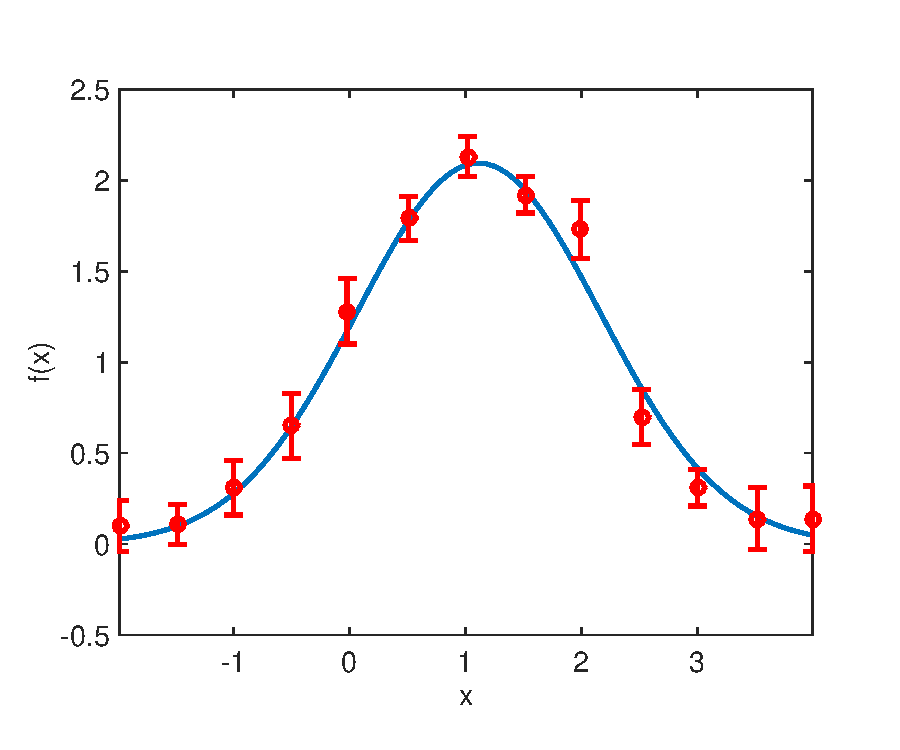
\includegraphics[width=2.5in]{19.Optimization/ga_gauss.pdf}
\caption{The noisy data (Table \ref{tbl:Gaussian}) is plotted with red circles with the error bars.  The solid line is the result of the optimization using the genetic algorithm.}
\label{fig:ga_gauss}
\end{figure}

In Chapter 11, we fitted a noisy data with a Lorentzian function using the nonlinear least square fitting method (See Example 11.5). It worked very well.  However, since the nonlinear $\chi^2$ function can have multiple minimums, the nonlinear least square fitting is not guaranteed to work.   If we tried to fit a noisy Gaussian like data with a single Gaussian function using the least square fitting method, most likely it fails.  The matrix becomes very close to singular and linear equation cannot be solve accurately by numerical methods.

The genetic algorithm does not suffer from such difficulties.  Consider a Gaussian function 
\begin{equation}
f(x;a,b,c) = a \me^{-(x-b)^2/c}
\end{equation}
where $a$, $b$, and $c$ are the parameters to be adjusted.  We want to fit the data set $\bar{f}_i$ with error $\sigma_i$ measured at $x_i$, $i=1, \cdots, M$ with the Gaussian function. The data is given in Table \ref{tbl:Gaussian}. As discussed in Chapter 11, the fitness function is given by
\begin{equation}
F(a,b,c) = \sum_i^K \left (f(x_i;a,b,c)-\bar{f}_i\right )^2/\sigma_i^2
\end{equation}
The $i$-the individual carries three genes, $x_j=(a_j, b_j, c_j)$ and the genes are bound by a lower and upper limit.  For example, $a_\text{min} < a_j < a_\text{max}$. The population consists of $N$ individuals as $p=(x_1, x_2, \cdots, x_N)$.  We use exactly the same algorithm as before.  It is noted that the inheritance rule is the same for all genes, that is
\begin{equation}
x_\text{child 1} = x_i + \xi (x_j-x_i), \quad x_\text{child 2} = x_j + \xi (x_i-x_j).
\end{equation} 
The same random number $\xi$ should be used for all genes so that the genes of offspring are between the parents' genes.
We use a slightly different mutation rule.  All members of the population are subject to the mutation at each generation cycle.  More than one members can be mutated at every generation cycle.



Program \ref{prog:ga_gauss} fits the noisy data with the Gaussian function.  The result is plotted in Fig. \ref{fig:ga_gauss}.
The fitting is quite reasonable.  After 3118 generations, we obtained the best gene $a=2.09$, $b=1.11$, $c=2.21$. This values could be further optimizaed by the steepest descent.  However, the fitting seems already good enough.

\subsection{Thomson problem}

Consider $N$ identical point charges $q$ placed on the surface of a sphere as shown in Fig. \ref{fig:thomson}.  The charges is free to move on the surface.  We want to know the lowest energy configuration of the charges. This problem is known as Thomson problem.\cite{thomson}  The lowest energy known at present is listed in WiKipedia for $N$=2 to 470.  We know the exact solution only for $N$=1--6 and 12.  For other sizes, it is not yet known that the observed lowest energy is actually the global minimum.  The Thomson problem is still an unsolved mathematical problem.  It is also important for physics, for example, in connection to the atomic structure.\cite{LaFave}.

We attempt to solve this problem numerically using the genetic algorithm.
The energy of the system is simply Coulomb energy
\begin{equation}
U(\vec{r}_1, \vec{r}_2, \cdots, \vec{r}_N) =  \frac{q}{4 \pi \epsilon_0} \sum_{i>j} \frac{1}{|\vec{r}_i - \vec{r}_j|}
\end{equation}
where $\vec{r}_i$ is the position vector for the $i$-th charge and its component is expressed in a spherical coordinate
\begin{equation}
x_i = R \sin\theta_i \cos\phi_i, \quad y_i=R \sin\theta_i \sin\phi_i, \qquad z_i = R \cos\theta_i
\end{equation}
where $R$ is the radius of the sphere and $\theta_i$ and $\phi_i$ are elevation and azimuthal angles.

To find the global minimum of energy, we use the potential energy as a fitness function and optimize it with respect to the angular variables using the genetic algorithm.
Since the global rotation does not change the energy, we set
\begin{equation}
\theta_1=0, \quad \phi_1=\phi_2=0.
\end{equation}
Hence, the number of variables (genes) is $2N-3$.
This fitness function has many local minimums very close to the global minimum and thus the finding the global minimum is challenging.  For $N=5$, the answer is known to be $E(5)=6.474691495$.  For $N=8$, $E(8)=19.675$ is the lowest energy discovered up-to-now.  

The simple mutation we used does not work well for the present problem. In Program \ref{prog:thomson}, the mutation rate changes randomly, occasionally the mutation rates jumps to a high value. It turns out that this burst of the mutation improves the optimization significantly.  We assume that the mutation rate bursts every ten generations.\footnote{This significant improvement was noted by Alex Skinner who took this course in 2014.}

For $N=5$, we find $E(5)=6.4746914947$ and the configuration is triangular dipyramid ($D_{3h}$) in perfect agreement with known results.

\begin{figure}
\centering
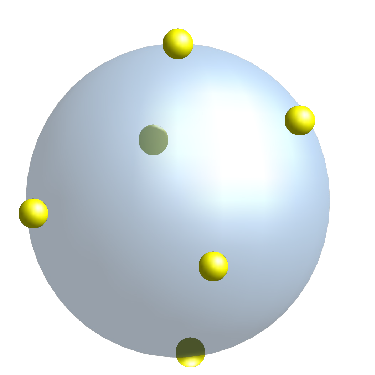
\includegraphics[width=1.5in]{19.Optimization/thomson.pdf}
\caption{Thomson problem:  Place $N$ point charges on the surface of a sphere such that the electrostatic potential energy is at the global minimum.}
\label{fig:thomson} 
\end{figure}

\newpage
\noindent
\section{Problems}

\begin{enumerate}[labelwidth=0.5cm,labelindent=0cm,leftmargin=*,label=\bfseries \thechapter.\arabic*,align=left]
\item
In Example \ref{ex:global_harmonic_coupling}, we constructed a fitness function for a fictitious molecule where all atoms are connected by identical springs.  Find the lowest energy structure for $N=5$.

\end{enumerate}

\newpage
\noindent
\section*{MATLAB Source Codes}
\addcontentsline{toc}{section}{\protect\numberline{}MATLAB Source Codes}


\noindent
\program
\label{prog:sa}
\footnotesize
\begin{verbatim}
%**************************************************************************
%*     Example 19.2                                                       *
%*     filename: ch19pr01.m                                               *
%*     program listing number: 19.1                                       *
%*                                                                        *
%*     This program attempt to find a grobal minimum of a fitness         *
%*     function U(x) using simulated annealing.                                         *
%*                                                                        *
%*     Programed by Ryoichi Kawai for Computational Physics Course.       *
%*     Last modification:  04/01/2017.                                    *
%**************************************************************************
close all
clc

L=241; % size of the descretized configuration space
dx=0.1;
xmin=(121-L)*dx; % bound of the configuration space
xmax=(L-121)*dx;
x=linspace(xmin,xmax,L);

% fitness function
U=@(x) -3.*cos(2.*x)+0.2*x.^2+3.0;

% graphics parameter
movie=false;  % movie slows down the simulation

NP=2^3;  % population size
p=rand(NP,1)*(xmax-xmin)+xmin;  % initial configuration
T=5; % initial temperature
E=U(p); % initial fitness
dp=0.1; % Metropolis max step length

NT=200; % Total cooling steps
NS=2000; % Total thermalization steps
RT=0.98; % Cooling rate

if movie
    figure(1)
    set(gcf,'units','inches','position',[1,1,6,5])
end

for k=1:NT % Cooling Loop
    temp(k)=T;

    for i=1:NS % Thermalization Loop (Metropolis)
        
        for j=1:NP % Loop over population

            found=false;
            while not(found)
                p0=p(j)+(1-2*rand(1))*dp;
                E0=U(p0);
                if exp(-(E0-E(j))/T) > rand(1)
                    found=true;
                    if p0<xmin || p0>xmax
                        p(j)=rand(1)*(xmax-xmin)+xmin;
                        E(j)=U(p(j));
                    else
                        p(j)=p0;
                        E(j)=E0;
                    end
                end
            end
        end

        if movie && mod(i,10)==0 % update movie
            plot(x,U(x))
            xlim([xmin,xmax])
            ylim([-1,19])
            hold on
            for j=1:NP
                rectangle('Position',[p(j)-0.25,U(p(j))-0.25,0.5,0.5],...
                    'Curvature',[1 1],'FaceColor','b');
            end
            drawnow
            hold off
        end

    end
    Emin(k)=min(E);
    fprintf('T=%f,   Emin=%f\n',T,Emin(k))
    
    T=T*0.98; % Exponential cooling schedule
end

fprintf('Final Temperature = %d\n',temp(200));
fprintf('Final Lowest Fitness = %d\n', Emin(200));
    
figure(1)
q=plot(x,U(x));
xlim([xmin,xmax])
ylim([-1,19])
xlabel('x','fontsize',14)
ylabel('Fitness','fontsize',14)
hold on
for j=1:NP
	rectangle('Position',[p(j)-0.25,U(p(j))-0.25,0.5,0.5],'Curvature',[1 1]);
end
drawnow
hold off

figure(2)
q=plot([1:200],temp,[1:200],Emin);
set(q(1),'color','black')
set(q(2),'color','red')
ylim([-2,6]);
xlabel('Steps','fontsize',14)
ylabel('Temperature/Lowest Fitness Value','fontsize',14)
legend('Temperature','Lowest Fitness Value')
\end{verbatim}
\normalsize


\ruleend

\bigskip
\noindent
\program
\label{prog:ga}
\footnotesize
\begin{verbatim}
%**************************************************************************
%*     Example 19.3                                                       *
%*     filename: ch19pr02.m                                               *
%*     program listing number: 19.2                                       *
%*                                                                        *
%*     This program findw a grobal minimum of a fitness function U(x)     *
%*     using genetic algorithm.                                           *
%*                                                                        *
%*     Programed by Ryoichi Kawai for Computational Physics Course.       *
%*     Last modification:  04/01/2017.                                    *
%**************************************************************************
close all

L=121; % size of the descretized configuration space
dx=0.1;
xmin=0; % bound of the configuration space
xmax=(L-1)*dx;
x=[0:L-1]*dx;
U=@(x) cos(5*x)-2*sin(3.5*x)+0.5*cos(x+0.5)+4; % fitness function

% parameter sof genetic algorithm
N=2^8; % size of population
p=rand(N,1)*xmax; % initial population
max_count=100; % waiting time
mutaion=0.1;  % mutation rate (fixed)

% initial fitness
f=U(p);
[f_sort,ix]=sort(f);
fmin=f_sort(1);
q=p(ix);  % q=individual in the order of their fitness



% plot initial population
figure(1)
set(gcf,'units','inches','position',[1,1,6,6])
plot(x,U(x))
axis([xmin xmax -1 11])
hold on
for i=1:N;
    rectangle('Position',[p(i)-0.2,U(p(i))-0.2,0.4,0.4],'Curvature',[1 1]);
end
drawnow
hold off

count=0;
found=false;
ip=zeros(N/2,1);
generation=0;

while not(found)
    generation=generation+1;
    pause(0.1)
    %%%%%%%%%%%%%%%%%%%%%%%%%%%%%%%%%%%%%%%%%%%%%%%%%%%%%%%%%%%%%%%%
    % select mating pairs from survivors (Knuth shuffle)
    for i=1:N/2
        j=ceil(rand(1)*i);
        ip(i)=ip(j);
        ip(j)=i;
    end
    % The following MATLAB builtin function can be used in place for
    % the above Knuth shuffle
    % ip=randperm(N/2);  
    %%%%%%%%%%%%%%%%%%%%%%%%%%%%%%%%%%%%%%%%%%%%%%%%%%%%%%%%%%%%%%%%%
    
    % generate offspring
    for k=1:2:N/2

        i=ip(k);
        j=ip(k+1);
        g=rand(2);
       
        % replace the deads with the new borns
        q(k+1+N/2)= q(i)+g(1)*(q(j)-q(i)+0.01);  % inheritance
        q(k+2+N/2)= q(j)+g(2)*(q(i)-q(j)+0.01);  % inheritance
    end
    
    % mutation
    if mod(generation,10)==0
        mutation=0.8;
    else
        mutation=0.1;
    end
    if rand(1)<mutaion
        i=ceil(rand(1)*N);
        q(i)=rand(1)*xmax;
    end
    
    p=q; % store new population
    
    % evaluate fitness
    f=U(p);
    % plot the current generation
    plot(x,U(x))
    axis([xmin xmax -1 11])
    hold on
    for i=1:N;
        rectangle('Position',[p(i)-0.2,U(p(i))-0.2,0.4,0.4],'Curvature',[1 1]);
    end
    drawnow
    pause(0.5);
    hold off

    %  sort the population
    [f_sort,ix]=sort(f);
    q=p(ix);
    
    % check if converged
    if f_sort(1)>=fmin
        count=count+1;
        if count > max_count
            found=true;  % waited long enough
        end
    else
        count=0; % reset wating couter
        fmin=f_sort(1);
        fprintf('New low found: generation=%d fitness=%.15f\n',generation,fmin)
    end
    
    bestfit(generation)=fmin;

end

fprintf('optimal x=%f,   U(x)=%f\n',q(1),f_sort(1))

figure(2)
plot([1:generation],bestfit(1:generation),'-or')
hold on
axis([0 generation 0.4 1]) 
xlabel('Generation','fontsize',14)
ylabel('Best Finess','fontsize',14)
\end{verbatim}
\normalsize

\ruleend

\bigskip
\noindent
\program
\label{prog:ga_gauss}
\footnotesize
\begin{verbatim}
%**************************************************************************
%*     Section 19.4.1                                                     *
%*     filename: ch19pr03.m                                               *
%*     program listing number: 19.3                                       *
%*                                                                        *
%*     This program fits a Gaussian disitrbution to a noisy data set      *
%*     using genetic algorithm.                                           *
%*                                                                        *
%*     Programed by Ryoichi Kawai for Computational Physics Course.       *
%*     Last modification:  04/02/2017.                                    *
%**************************************************************************


% Generate an experimental data set
N=13;
x=[-1.98,-1.48,-1.00,-0.50,-0.02,0.51,1.02,1.52,1.99,2.52,3.00,3.52,3.99];
y=[ 0.10, 0.11, 0.31, 0.65, 1.28,1.79,2.13,1.92,1.73,0.70,0.31,0.14,0.14];
s=[ 0.14, 0.11, 0.15, 0.18, 0.18,0.12,0.11,0.10,0.16,0.15,0.10,0.17,0.18];

% theoretical data space
K=101;
dx=(x(N)-x(1))/(K-1);
X=linspace(x(1),x(N),K);

% control parameter for genetic algorithm
NP=2^10;
MP=int32(NP/2);
max_count=200;
max_generation=10000;

% parameter spce (genes)
a_max=5; a_min=0;
b_max=5; b_min=-5;
c_max=5; c_min=0.01;

% initial parameters (genes)
a=rand(NP,1)*(a_max-a_min)+a_min;
b=rand(NP,1)*(b_max-b_min)+b_min;
c=rand(NP,1)*(c_max-c_min)+c_min;

%  allocate arrays
ip=zeros(1,MP);
F=zeros(1,NP);
G=zeros(N,NP);

% graphics setting
close all;
movie = true;
if movie
    figure(1);
    axis([x(1) x(end) -0.5 2.5]);
end

% reset the counters
found=false;
count=0;
generation=0;
Fmin=realmax();   % some large number

% genetic evolution begins here
while not(found)
    
    generation=generation+1;
    if generation > max_generation  % too many generations
        fprintf('Max generation reached.  Terminated.\n');
        break;
    end
    
    % eveluate the initial fitness
    for i=1:NP
        for j=1:N
            G(j,i)=a(i)*exp(-(x(j)-b(i))^2/c(i));
        end
        F(i)=sum((G(:,i)-y(:)).^2./s(:))/N;
    end
 
    % sort the population based on thier fitness
    [Fs, IX]=sort(F);
    as=a(IX); bs=b(IX); cs=c(IX);

    if movie
        % plot current best fitting
        Y=as(1)*exp(-(X-bs(1)).^2/cs(1));
        r=plot(X,Y);
        set(r,'linewidth',2)
        hold on
        r=errorbar(x,y,s,'o');
        set(r,'linewidth',2,'color','red')
        xlabel('x','fontsize',14)
        ylabel('f(x)','fontsize',14)
        hold off
        axis([x(1) x(N) -0.5 2.5]);
        drawnow
        pause(0.2)
    end
    
    % check if converged
    if Fs(1)>=Fmin
        count=count+1;
        if count > max_count  % exceed the waiting time limit
            found=true;
            break
        end
    else
        count=0;            %reset wating time counter
        Fmin=Fs(1);         % new lowest fitness
        a0=as(1); b0=bs(1); c0=cs(1);
        fprintf('New low found: generation=%i, fitness= %.15f, a=%f, b=%f, c=%f\n',...
            generation,Fmin,a0,b0,c0)
    end
    
    % find mating pairs from the survived population
    ip=randperm(MP); 
    
    % generate offsprings
    for k=1:2:MP
        g=rand(6);
        i=ip(k);
        j=ip(k+1);
        as(k+1+NP/2)= as(i)+g(1)*(as(j)-as(i)+0.01);
        as(k+2+NP/2)= as(j)+g(2)*(as(i)-as(j)+0.01);
        bs(k+1+NP/2)= bs(i)+g(3)*(bs(j)-bs(i)+0.01);
        bs(k+2+NP/2)= bs(j)+g(4)*(bs(i)-bs(j)+0.01);
        cs(k+1+NP/2)= cs(i)+g(5)*(cs(j)-cs(i)+0.01);
        cs(k+2+NP/2)= cs(j)+g(6)*(cs(i)-cs(j)+0.01);
    end
 
    % mutation rate (every 10 generations, mutation burst happens
    if mod(generation,10)==0
        mutation=0.8;
    else
        mutation=0.1;
    end
    
    %  mutation
    rm=rand(1,NP);
    for i=2:NP
        if rm(i)<mutation
            as(i)=rand(1)*(a_max-a_min)+a_min;
            bs(i)=rand(1)*(b_max-b_min)+b_min;
            cs(i)=rand(1)*(c_max-c_min)+c_min;
        end
    end
    
    % store genes of new population
    a=as; b=bs; c=cs;
 
end
    
fprintf('Best fit=%.15f,  a=%f, b=%f, c=%f\n',Fmin,a0,b0,c0)

% plot the best fitting
if not(movie)
    figure(1);
    axis([x(1) x(end) -0.5 2.5])
end

Y=a0*exp(-(X-b0).^2/c0);
r=plot(X,Y);
set(r,'linewidth',2)
hold on
r=errorbar(x,y,s,'o');
set(r,'linewidth',2,'color','red')
xlabel('x','fontsize',14)
ylabel('f(x)','fontsize',14)
axis([x(1) x(N) -0.5 2.5]);
hold off
drawnow
\end{verbatim}
\normalsize

\ruleend

\bigskip
\noindent
\program
\label{prog:thomson}
\footnotesize
\begin{verbatim}
%**************************************************************************
%*     Section 19.4.2                                                     *
%*     filename: ch19pr04.m                                               *
%*     program listing number: 19.4                                       *
%*                                                                        *
%*     This program solves the Thomson problem  using genetic algorithm.  *
%*     using genetic algorithm.                                           *
%*                                                                        *
%*     Programed by Ryoichi Kawai for Computational Physics Course.       *
%*     Improved by Alex Skinner.                                          *
%*     Last modification:  04/02/2017.                                    *
%**************************************************************************
clear all;

% system parameters
N=5;
R=1;

% parameters for genetic algorithm
NP=2^12;          % population size
MP=int32(NP/2);   % half of the population
max_count=200;    % stopping condition
max_generation=10000;   % maximum generation

% parameter space (genes)
th_max=pi; th_min=0;
ph_max=2*pi; ph_min=0;

% initial parameters (genes)
th=rand(N,NP)*(th_max-th_min)+th_min;
ph=rand(N,NP)*(ph_max-ph_min)+ph_min;
th(1,:)=0;
ph(1,:)=0;
ph(2,:)=0;
th(3,1)=th_max;
ph(3,2)=ph_max;

% allocate arrays
ip=zeros(1,MP);
F=zeros(1,NP);
phs=zeros(N,NP);
ths=zeros(N,NP);

% reset the counters
found=false;
count=0;
generation=0;
Fmin=realmax();

% genetic evolution begins here
while not(found)

    generation=generation+1;
    if generation > max_generation  % too many generations
        fprintf('Max generation reached.  Terminated.\n')
        break;
    end
    
    % eveluate the initial fitness
    for i=1:NP
        F(i)=UCoulomb(th(:,i),ph(:,i),R);
    end
 
    % sort the population based on thier fitness
    [Fs, IX]=sort(F);
    ths=th(:,IX); phs=ph(:,IX); 
     
    % check if converged
    if Fs(1)>=Fmin
        count=count+1;
        if count > max_count  % exceed the waiting time limit
            found=true;
            break
        end
    else
        count=0; %reset wating time counter
        Fmin=Fs(1);
        fprintf('New low found: generation=%i, fitness= %.15f\n',generation,Fmin)
    end
    
    % find mating pairs from the survived population
    ip=randperm(MP);
    
    % generate offsprings       
    for k=1:2:NP/2
        % g ranges from -1 to 1
        g=-2*rand(2)+1;
        i=ip(k);
        j=ip(k+1);
        ths(:,k+1+MP)= ths(:,i)+g(1)*(ths(:,j)-ths(:,i));
        ths(:,k+2+MP)= ths(:,j)+g(2)*(ths(:,i)-ths(:,j));
        phs(:,k+1+MP)= phs(:,i)+g(1)*(phs(:,j)-phs(:,i));
        phs(:,k+2+MP)= phs(:,j)+g(2)*(phs(:,i)-phs(:,j));
    end
  
    % mutation rate         
    if mod(generation,10)==0
        mutation=0.8*rand();
    else
        mutation=0.3*rand();
    end
    
    % mutation  
    rm=rand(NP,1);
    for i=2:NP
        if rm(i)<mutation
            ths(:,i)=rand(N,1)*(th_max-th_min)+th_min;
            phs(:,i)=rand(N,1)*(ph_max-ph_min)+ph_min;
            ths(1,i)=0;
            phs(1:2,i)=0;
       end
    end
    
    % store new population
    th=ths; ph=phs;
end

fprintf('Lowest Energy=%.15f\n',Fmin)
for i=1:N
    fprintf('theta=%f, phi=%f\n',ths(i),phs(i))
end

for i=1:N
    X(i)=R*sin(ths(i,1))*cos(phs(i,1));
    Y(i)=R*sin(ths(i,1))*sin(phs(i,1));
    Z(i)=R*cos(ths(i,1));
end

close all;
figure(1)
plot3(X,Y,Z,'o')
axis equal;
xlim([-1,1]);
ylim([-1,1]);
zlim([-1,1]);
grid on
hold on
drawnow

bond=10.0;
for i=1:N
    for j=i+1:N
        d=sqrt((X(i)-X(j))^2+(Y(i)-Y(j))^2+(Z(i)-Z(j))^2);
        bond = min(bond,d);
    end
end
bond=bond*1.25;
for i=1:N
    for j=i+1:N
        d=sqrt((X(i)-X(j))^2+(Y(i)-Y(j))^2+(Z(i)-Z(j))^2);
        if d <= bond
            line([X(i),X(j)],[Y(i),Y(j)],[Z(i),Z(j)]);
            drawnow;
        end
    end
end
hold off
\end{verbatim}

\medskip
\footnotesize
\begin{verbatim}
%**************************************************************************
%*     filename: UCoulomb.m                                               *
%*                                                                        *
%*     Function called by ch19pr04.m                                      *
%**************************************************************************
function UC=UCoulomb(theta,phi,r)

N=size(theta,1);
UC=0;
X=sin(theta).*cos(phi);
Y=sin(theta).*sin(phi);
Z=cos(theta);
for i=1:N
    for j=i+1:N
        r12=sqrt((X(i)-X(j))^2+(Y(i)-Y(j))^2+(Z(i)-Z(j))^2);
        UC=UC+1.0/(r12*r);
    end
end
\end{verbatim}
\normalsize

\ruleend

\bigskip
\noindent
\section*{Python Source Codes}
\addcontentsline{toc}{section}{\protect\numberline{}Python Source Codes}
\setcounter{program}{0}

\bigskip
\noindent
\program
\footnotesize
\begin{verbatim}
#!/usr/bin/env python3
# -*- coding: utf-8 -*-
"""
%**************************************************************************
%*     Example 19.2                                                       *
%*     filename: ch19pr01.py                                              *
%*     program listing number: 19.1                                       *
%*                                                                        *
%*     This program attempt to find a grobal minimum of a fitness         *
%*     function U(x) using simulated annealing.                                         *
%*                                                                        *
%*     Programed by Ryoichi Kawai for Computational Physics Course.       *
%*     Last modification:  04/01/2017.                                    *
%**************************************************************************
"""
import numpy as np
import matplotlib.pyplot as plt

plt.close('all')

# system setting
L=241    # size of the descretized configuration space
dx=0.1   # grid size
xmin=0.0 # lower bound of the configuration space
xmax=(L-1)*dx  # upper boound
x=np.linspace(xmin,xmax,L)

def U(x):  # fitness function
    return -3.*np.cos(2.*(x-xmax/2.))+0.2*(x-xmax/2.)**2+3.0

# graphics parameter
movie=False   # show animation

NP=2**3   # population size
p=np.random.rand(NP)*(xmax-xmin)+xmin # initial configuration
T=5.0 # initial temperature
E=U(p)  # initial fitness
dp=0.1  # Metropolis max step length

NT=200   # Total cooling steps
NS=2000  # Total thermalization steps
RT=0.98  # Cooling rate

# allocate arrayss
temp=np.zeros(NT)
Emin=np.zeros(NT)

if movie:
    plt.figure(figsize=(6,5))
    
for k in range(0,NT): # loop over time step
    temp[k]=T

    for i in range(0,NS): # Thermalization Loop (Metropolis)
        
        for j in range(0,NP):  # Loop over population

            found=False
            while not(found):
                p0=p[j]+np.random.choice([-1,1])*dp
                E0=U(p0)
                if np.exp(-(E0-E[j])/T) > np.random.rand(1):
                    found=True
                    if p0<xmin or p0>xmax:
                        p[j]=np.random.rand(1)*(xmax-xmin)+xmin
                        E[j]=U(p[j])
                    else:
                        p[j]=p0
                        E[j]=E0

        if movie: # update movie
            plt.clf()
            plt.plot(x,U(x))
            plt.xlim([xmin,xmax])
            plt.ylim([-1,19])

            for j in range(0,NP):
                circle=plt.Circle((p[j],U(p[j])),0.25,fc='b')
                plt.gca().add_patch(circle)
                plt.pause(0.0001)

    Emin[k]=np.min(E)
    print('T={0:f},   Emin={1:f}'.format(T,Emin[k]))
    
    T=T*0.98  # Exponential cooling schedule

print('Final Temperature = {0:f}'.format(temp[k]))
print('Final Lowest Fitness = {0:f}'.format(Emin[k]))
    
if not(movie):
    plt.figure(figsize=(6,5))
    plt.plot(x,U(x))
    plt.xlim([xmin,xmax])
    plt.ylim([-1,19])

    for j in range(0,NP):
        circle=plt.Circle((p[j],U(p[j])),0.25,fc='b')
        plt.gca().add_patch(circle)
        plt.pause(0.0001)

plt.xlabel('x',fontsize=14)
plt.ylabel('Fitness',fontsize=14)
plt.show()
    
plt.figure(figsize=(6,5))
t=np.linspace(1,NT,NT)
plt.plot(t,temp,'-k',label='temperature')
plt.plot(t,Emin,'-r',label='energy')
plt.xlabel('Steps',fontsize=14)
plt.ylabel('Energy',fontsize=14)
plt.legend(loc=1)
plt.show()
\end{verbatim}
\normalsize

\ruleend

\bigskip
\noindent
\program
\footnotesize
\begin{verbatim}
#!/usr/bin/env python3
# -*- coding: utf-8 -*-
"""
%**************************************************************************
%*     Example 19.3                                                       *
%*     filename: ch19pr02.py                                              *
%*     program listing number: 19.2                                       *
%*                                                                        *
%*     This program findw a grobal minimum of a fitness function U(x)     *
%*     using genetic algorithm.                                           *
%*                                                                        *
%*     Programed by Ryoichi Kawai for Computational Physics Course.       *
%*     Last modification:  04/01/2017.                                    *
%**************************************************************************
"""
import numpy as np
import matplotlib.pyplot as plt
plt.close('all')

#system configuration
L=121          # size of the descretized configuration space
dx=0.1         # grid size
xmin=0.0       # lower bound of the configuration space
xmax=(L-1)*dx  # upper bound
x=np.linspace(xmin,xmax,L)

def U(x): # fitness function
    return np.cos(5.0*x)-2.0*np.sin(3.5*x)+0.5*np.cos(x+0.5)+4.0 

# parameter sof genetic algorithm
N=2**8            # size of population
M=np.int(N/2)
p=np.random.rand(N)*xmax  # initial population

max_count=100     # waiting time
mutaion=0.1       # mutation rate (fixed)
max_generation=10000
bestfit=np.zeros(max_generation)

# initial fitness
f=U(p)  # fitness
ix=np.argsort(f)   # sorting population basd on their fitness
fmin=f[ix[0]] 
q=p[ix]
bestfit[0]=fmin

# plot initial population
plt.figure(figsize=(6,6))
plt.plot(x,U(x))
plt.xlim([xmin, xmax])
plt.ylim([-1, 11])
plt.axis('equal')

for i in range(0,N):
    circle=plt.Circle((p[i],U(p[i])),0.2,facecolor='none', edgecolor='b')
    plt.gca().add_patch(circle)
plt.pause(0.0001)

count=0;
found=False
ip=np.zeros(M)
generation=0;

while not(found):
    generation=generation+1
    if generation > max_generation:
        print('Max generation reached.  Terminated.')
        break
    
    ip=np.random.permutation(M)  
    
    # generate offspring
    for k in range(0,M,2):

        i=ip[k]
        j=ip[k+1]
        g=np.random.rand(2)
        # replace the deads with the new borns
        q[k+M]= q[i]+g[0]*(q[j]-q[i]+0.01)     # inheritance
        q[k+1+M]= q[j]+g[1]*(q[i]-q[j]+0.01)  # inheritance
    
    # mutation
    if np.mod(generation,10)==0:
        mutation=0.8
    else:
        mutation=0.1
    
    if np.random.rand(1)<mutaion:
        i=np.random.randint(0,N)
        q[i]=np.random.rand(1)*(xmax-xmin)

    p=q  # store new population
    
    # evaluate fitness
    f=U(p)
    plt.clf()
    plt.plot(x,U(x))
    plt.xlim([xmin, xmax])
    plt.ylim([-1, 11])

    for i in range(0,N):
        circle=plt.Circle((p[i],U(p[i])),0.2,facecolor='none', edgecolor='b')
        plt.gca().add_patch(circle)
    plt.pause(0.0001)

    #  sort the population
    ix=np.argsort(f)
    q=p[ix]
    
    #check if converged
    if f[ix[0]]>=fmin :
        count=count+1
        if count > max_count:
            found=True  # waited long enough

    else:
        count=0  # reset wating couter
        fmin=f[ix[0]]
        print('New low found: generation={0:d} fitness={1:.15f}'.format(generation,fmin))

    bestfit[generation]=fmin

print('optimal x={0:f},   U(x)={1:f}'.format(q[0],f[ix[0]]))

plt.figure(figsize=(6,5))
t=np.linspace(0,generation,generation+1)
plt.plot(t,bestfit[0:generation+1],'-or',mfc=None)
plt.xlabel('Generation',fontsize=14)
plt.ylabel('Best Finess',fontsize=14)
plt.show()
\end{verbatim}
\normalsize

\ruleend

\bigskip
\noindent
\program
\footnotesize
\begin{verbatim}
#!/usr/bin/env python3
# -*- coding: utf-8 -*-
"""
%**************************************************************************
%*     Section 19.4.1                                                     *
%*     filename: ch19pr03.m                                               *
%*     program listing number: 19.3                                       *
%*                                                                        *
%*     This program fits a Gaussian disitrbution to a noisy data set      *
%*     using genetic algorithm.                                           *
%*                                                                        *
%*     Programed by Ryoichi Kawai for Computational Physics Course.       *
%*     Last modification:  04/02/2017.                                    *
%**************************************************************************
"""
import numpy as np
import matplotlib.pyplot as plt

# sample experimental data set
N=13
x=[-1.98,-1.48,-1.00,-0.50,-0.02,0.51,1.02,1.52,1.99,2.52,3.00,3.52,3.99]
y=[ 0.10, 0.11, 0.31, 0.65, 1.28,1.79,2.13,1.92,1.73,0.70,0.31,0.14,0.14]
s=[ 0.14, 0.11, 0.15, 0.18, 0.18,0.12,0.11,0.10,0.16,0.15,0.10,0.17,0.18]

# theoretical data space
K=101
X=np.linspace(x[0],x[-1],K)

# control parameter for genetic algorithm
NP=2**10           # population size
MP=np.int(NP/2)   # half of the population
max_count=200     # stopping condition
max_generation=10000   # maximum generation

# parameter space (genes)
a_max=5.0; a_min=0.0
b_max=5.0; b_min=-5.0
c_max=5.0; c_min=0.01

# initial parameters (genes)
a=np.random.rand(NP)*(a_max-a_min)+a_min
b=np.random.rand(NP)*(b_max-b_min)+b_min
c=np.random.rand(NP)*(c_max-c_min)+c_min

# allocate arrays
ip=np.zeros(MP)
F=np.zeros(NP)
G=np.zeros((N,NP))

# graphics setting
plt.close('all')
movie = True
if movie:
    plt.figure(figsize=(6,5))
    plt.axis([x[0], x[-1], -0.5, 2.5])
    
# reset the counters
found=False
count=0
generation=0
Fmin=np.finfo(np.float64()).max  # some large number 

# genetic evolution begins here
while not(found):
    
    generation=generation+1
    if generation > max_generation:  # too many generations
        print('Max generation reached.  Terminated.')
        break
    
    # eveluate the fitness
    for i in range(0,NP):
        for j in range(0,N):
            G[j,i]=a[i]*np.exp(-(x[j]-b[i])**2/c[i])
        F[i]=np.sum((G[:,i]-y[:])**2/s[:])/N

    # sort the population based on thier fitness
    IX=np.argsort(F)
    A=a[IX]; B=b[IX]; C=c[IX]
    
    if movie:
        #plot current best fitting
        plt.clf()
        Y=A[0]*np.exp(-(X-B[0])**2/C[0])
        plt.plot(X,Y,'-r',linewidth=2)
        plt.errorbar(x,y,yerr=s,fmt='ok')
        plt.pause(0.001)
    
    # check if converged
    if F[IX[0]]>=Fmin:
        count=count+1
        if count > max_count:  # no more evolution
            found=True
            break
    else:
        count=0;               # reset dewelling counter
        Fmin=F[IX[0]]          # new lowest fitness
        a0=A[0]; b0=B[0]; c0=C[0]  # current best genes
        print('New low found: generation={0:d}, fitness={1:.15f}, a={2:f}, b={3:f}, c={4:f}'.format(generation,Fmin,a0,b0,c0))

    # find mating pairs from the survived population
    ip=np.random.permutation(MP) 
     
    # generating oggsprings
    for k in range(0,MP,2):
        g=np.random.rand(6)
        i=ip[k]
        j=ip[k+1]
        A[k+MP]  = A[i]+g[0]*(A[j]-A[i]+0.01)
        A[k+MP+1]= A[j]+g[1]*(A[i]-A[j]+0.01)
        B[k+MP]  = B[i]+g[2]*(B[j]-B[i]+0.01)
        B[k+MP+1]= B[j]+g[3]*(B[i]-B[j]+0.01)
        C[k+MP]=   C[i]+g[4]*(C[j]-C[i]+0.01)
        C[k+MP+1]= C[j]+g[5]*(C[i]-C[j]+0.01)
 
    # mutation rate (every 10 generations, mutation burst happens)
    if np.mod(generation,10)==0:
        mutation=0.8
    else:
        mutation=0.1
        
    # mutation
    rm=np.random.rand(NP)
    for i in range(1,NP):
        if rm[i]<mutation:
            A[i]=np.random.rand(1)*(a_max-a_min)+a_min
            B[i]=np.random.rand(1)*(b_max-b_min)+b_min;
            C[i]=np.random.rand(1)*(c_max-c_min)+c_min;
    
    # store genes of new population
    a[:]=A[:]; b[:]=B[:]; c[:]=C[:]

print('Best fit:{0:.15f},  a={1:f},b={2:f}, c={3:f}'.format(Fmin, a0, b0, c0))

# plot the best fitting
if not(movie):
    plt.figure(figsize=(6,5))
    plt.axis([x[1], x[-1], -0.5, 2.5])
    
plt.clf()
Y=a0*np.exp(-(X-b0)**2/c0)
plt.plot(X,Y,'-r',linewidth=2)
plt.errorbar(x,y,yerr=s,fmt='ok')
plt.xlabel('x',fontsize=14)
plt.ylabel('f(x)',fontsize=14)
plt.show()
\end{verbatim}
\normalsize

\ruleend

\bigskip
\noindent
\program
\footnotesize
\begin{verbatim}
#!/usr/bin/env python3
# -*- coding: utf-8 -*-
"""
%**************************************************************************
%*     Section 19.4.2                                                     *
%*     filename: ch19pr04.m                                               *
%*     program listing number: 19.4                                       *
%*                                                                        *
%*     This program solves the Thomson problem  using genetic algorithm.  *
%*     using genetic algorithm.                                           *
%*                                                                        *
%*     Programed by Ryoichi Kawai for Computational Physics Course.       *
%*     Improved by Alex Skinner.                                          *
%*     Last modification:  04/02/2017.                                    *
%**************************************************************************
"""
import numpy as np
import matplotlib.pyplot as plt
from mpl_toolkits.mplot3d import Axes3D

# system parameters
N=5      # number of charges
R=1.0    # radius of the sphere

def U(theta,phi,r):  # potential energy (fitness function)
    u=0.0
    X=np.sin(theta)*np.cos(phi)
    Y=np.sin(theta)*np.sin(phi)    
    Z=np.cos(theta)    
    for i in range(0,N):
        for j in range(i+1,N):
            r12=np.sqrt((X[i]-X[j])**2+(Y[i]-Y[j])**2+(Z[i]-Z[j])**2)
            u=u+1.0/(r12*r)
    return u
    
# parameters for genetic algorithm
NP=2**12          # population size
MP=np.int(NP/2)   # half of the population
max_count=200;    # stopping condition
max_generation=10000   # maximum generation

# parameter space (genes)
th_max=np.pi; th_min=0.0
ph_max=2.0*np.pi; ph_min=0.0

# initial parameters (genes)
th=np.random.rand(N,NP)*(th_max-th_min)+th_min
ph=np.random.rand(N,NP)*(ph_max-ph_min)+ph_min
th[0,:]=0.0
ph[0,:]=0.0
ph[1,:]=0.0
th[2,0]=th_max
ph[2,1]=ph_max

# allocate arrays
ip=np.zeros(MP)
F=np.zeros(NP)
ths=np.zeros((N,NP))
phs=np.zeros((N,NP))

# reset the counters
found=False
count=0
generation=0
Fmin=np.finfo(np.float64()).max  # some large number 

# genetic evolution begins here
while not(found):
    
    generation=generation+1
    if generation > max_generation:  # too many generations
        print('Max generation reached.  Terminated.')
        break
    
    # eveluate the initial fitness
    for i in range(0,NP):
        F[i]=U(th[:,i],ph[:,i],R)
 
    # sort the population based on thier fitness
    IX=np.argsort(F)
    ths[:,:]=th[:,IX]; phs[:,:]=ph[:,IX] 
     
    # check if converged
    if F[IX[0]]>=Fmin:
        count=count+1
        if count > max_count:  # exceed the waiting time limit
            found=True
            break
    else:
        count=0   # reset wating time counter
        Fmin=F[IX[0]]
        print('New low found: generation={0:d}, fitness={1:.15f}'.format(generation,Fmin))
    
    # find mating pairs from the survived population
    ip=np.random.permutation(MP)
    
    # generate offsprings       
    for k in range(0,MP,2):
        # g ranges from -1 to 1
        g=-2.0*np.random.rand(2)+1.0
        i=ip[k]
        j=ip[k+1]
        ths[:,k+MP]  = ths[:,i]+g[0]*(ths[:,j]-ths[:,i])
        ths[:,k+1+MP]= ths[:,j]+g[1]*(ths[:,i]-ths[:,j])
        phs[:,k+MP]  = phs[:,i]+g[0]*(phs[:,j]-phs[:,i])
        phs[:,k+1+MP]= phs[:,j]+g[1]*(phs[:,i]-phs[:,j])

    # mutation rate              
    if np.mod(generation,10)==0:
        mutation=0.8*np.random.rand()
    else:
        mutation=0.3*np.random.rand()
        
    # mutation  
    rm=np.random.rand(NP)    
    for i in range(2,NP):
        if rm[i]<mutation:
            ths[:,i]=np.random.rand(N)*(th_max-th_min)+th_min
            phs[:,i]=np.random.rand(N)*(ph_max-ph_min)+ph_min
            ths[0,i]=0.0
            phs[0:1,i]=0.0
    
    # store new population
    th[:,:]=ths[:,:]; ph[:,:]=phs[:,:]

print('Lowest Energy={0:.15f}'.format(Fmin))
for i in range(0,N):
    print('theta={0:f}, phi={1:f}'.format(ths[i,0],phs[i,0]))

X=np.zeros(N)
Y=np.zeros(N)
Z=np.zeros(N)

for i in range(0,N):
    X[i]=R*np.sin(ths[i,0])*np.cos(phs[i,0])
    Y[i]=R*np.sin(ths[i,0])*np.sin(phs[i,0])
    Z[i]=R*np.cos(ths[i,0])

# plot 3D phase trajectory
plt.close('all')
fig=plt.figure()
ax=fig.gca(projection='3d')
plt.plot(X, Y, Z,'ob')
ax.set_xlabel('x')
ax.set_ylabel('y')
ax.set_zlabel('z')
ax.paspect=[1.0,1.0,1.0]
ax.set_xlim3d([-1.0,1.0])
ax.set_ylim3d([-1.0,1.0])
ax.set_zlim3d([-1.0,1.0])

bond=10.0
for i in range(0,N):
    for j in range(i+1,N):
        d=np.sqrt((X[i]-X[j])**2+(Y[i]-Y[j])**2+(Z[i]-Z[j])**2)
        bond = np.min([bond,d])

bond=bond*1.25
for i in range(0,N):
    for j in range(i+1,N):
        d=np.sqrt((X[i]-X[j])**2+(Y[i]-Y[j])**2+(Z[i]-Z[j])**2)
        if d <= bond:
            ax.plot([X[i],X[j]],[Y[i],Y[j]],[Z[i],Z[j]],'-b')
            plt.pause(0.0001)
plt.show()
\end{verbatim}
\normalsize

\ruleend
\vfill

\newpage
%\chapbibliography

\bibliographystyle{unsrt}
\bibliography{compphys}